% by pts@fazekas.hu at Fri Aug 28 09:29:30 CEST 2009
%
% SUXX: pdflatex cannot embed (missing glyph) a Keynote chart with an ff
%       ligature in the caption. Solution: ZERO-WIDH-JOINER unicode char.
\documentclass{beamer}
\usepackage{lmodern}
\usepackage{t1enc}
\usepackage{graphicx}
\usepackage{beamerthemesplit}

% !! EuroTeX 2009, town (subtitle?)
\title{Optimizing PDF output size of \TeX{} documents}
%\subtitle{blah}
\author{P\'eter Szab\'o}
\date{2009-08-31\par\medskip EuroTeX\,2009\\ The Hague, The Netherlands}

%** Put content to a frame with raggedbottom vertical alignment.
%** This has a hard-coded height for the useful content, depends on the
%** number of sections as well.
%** @example
%**   \frame{
%**      \nocenterframetitle{...}
%**      \nocenter{
%**      ...
%**      }
%**   }
\def\nocenter#1{%
  \hrule height0pt
  \vbox to200pt{\vsize=200pt{\ignorespaces#1}\vfil}%
}

\begin{document}

\frame{\titlepage}

\section[Outline]{}
\frame{\tableofcontents}

\section{Optimization effectiveness}

\subsection{Input PDF files used}

\frame{
\frametitle{Input PDF sizes}
\nocenter{%
\noindent\hfil
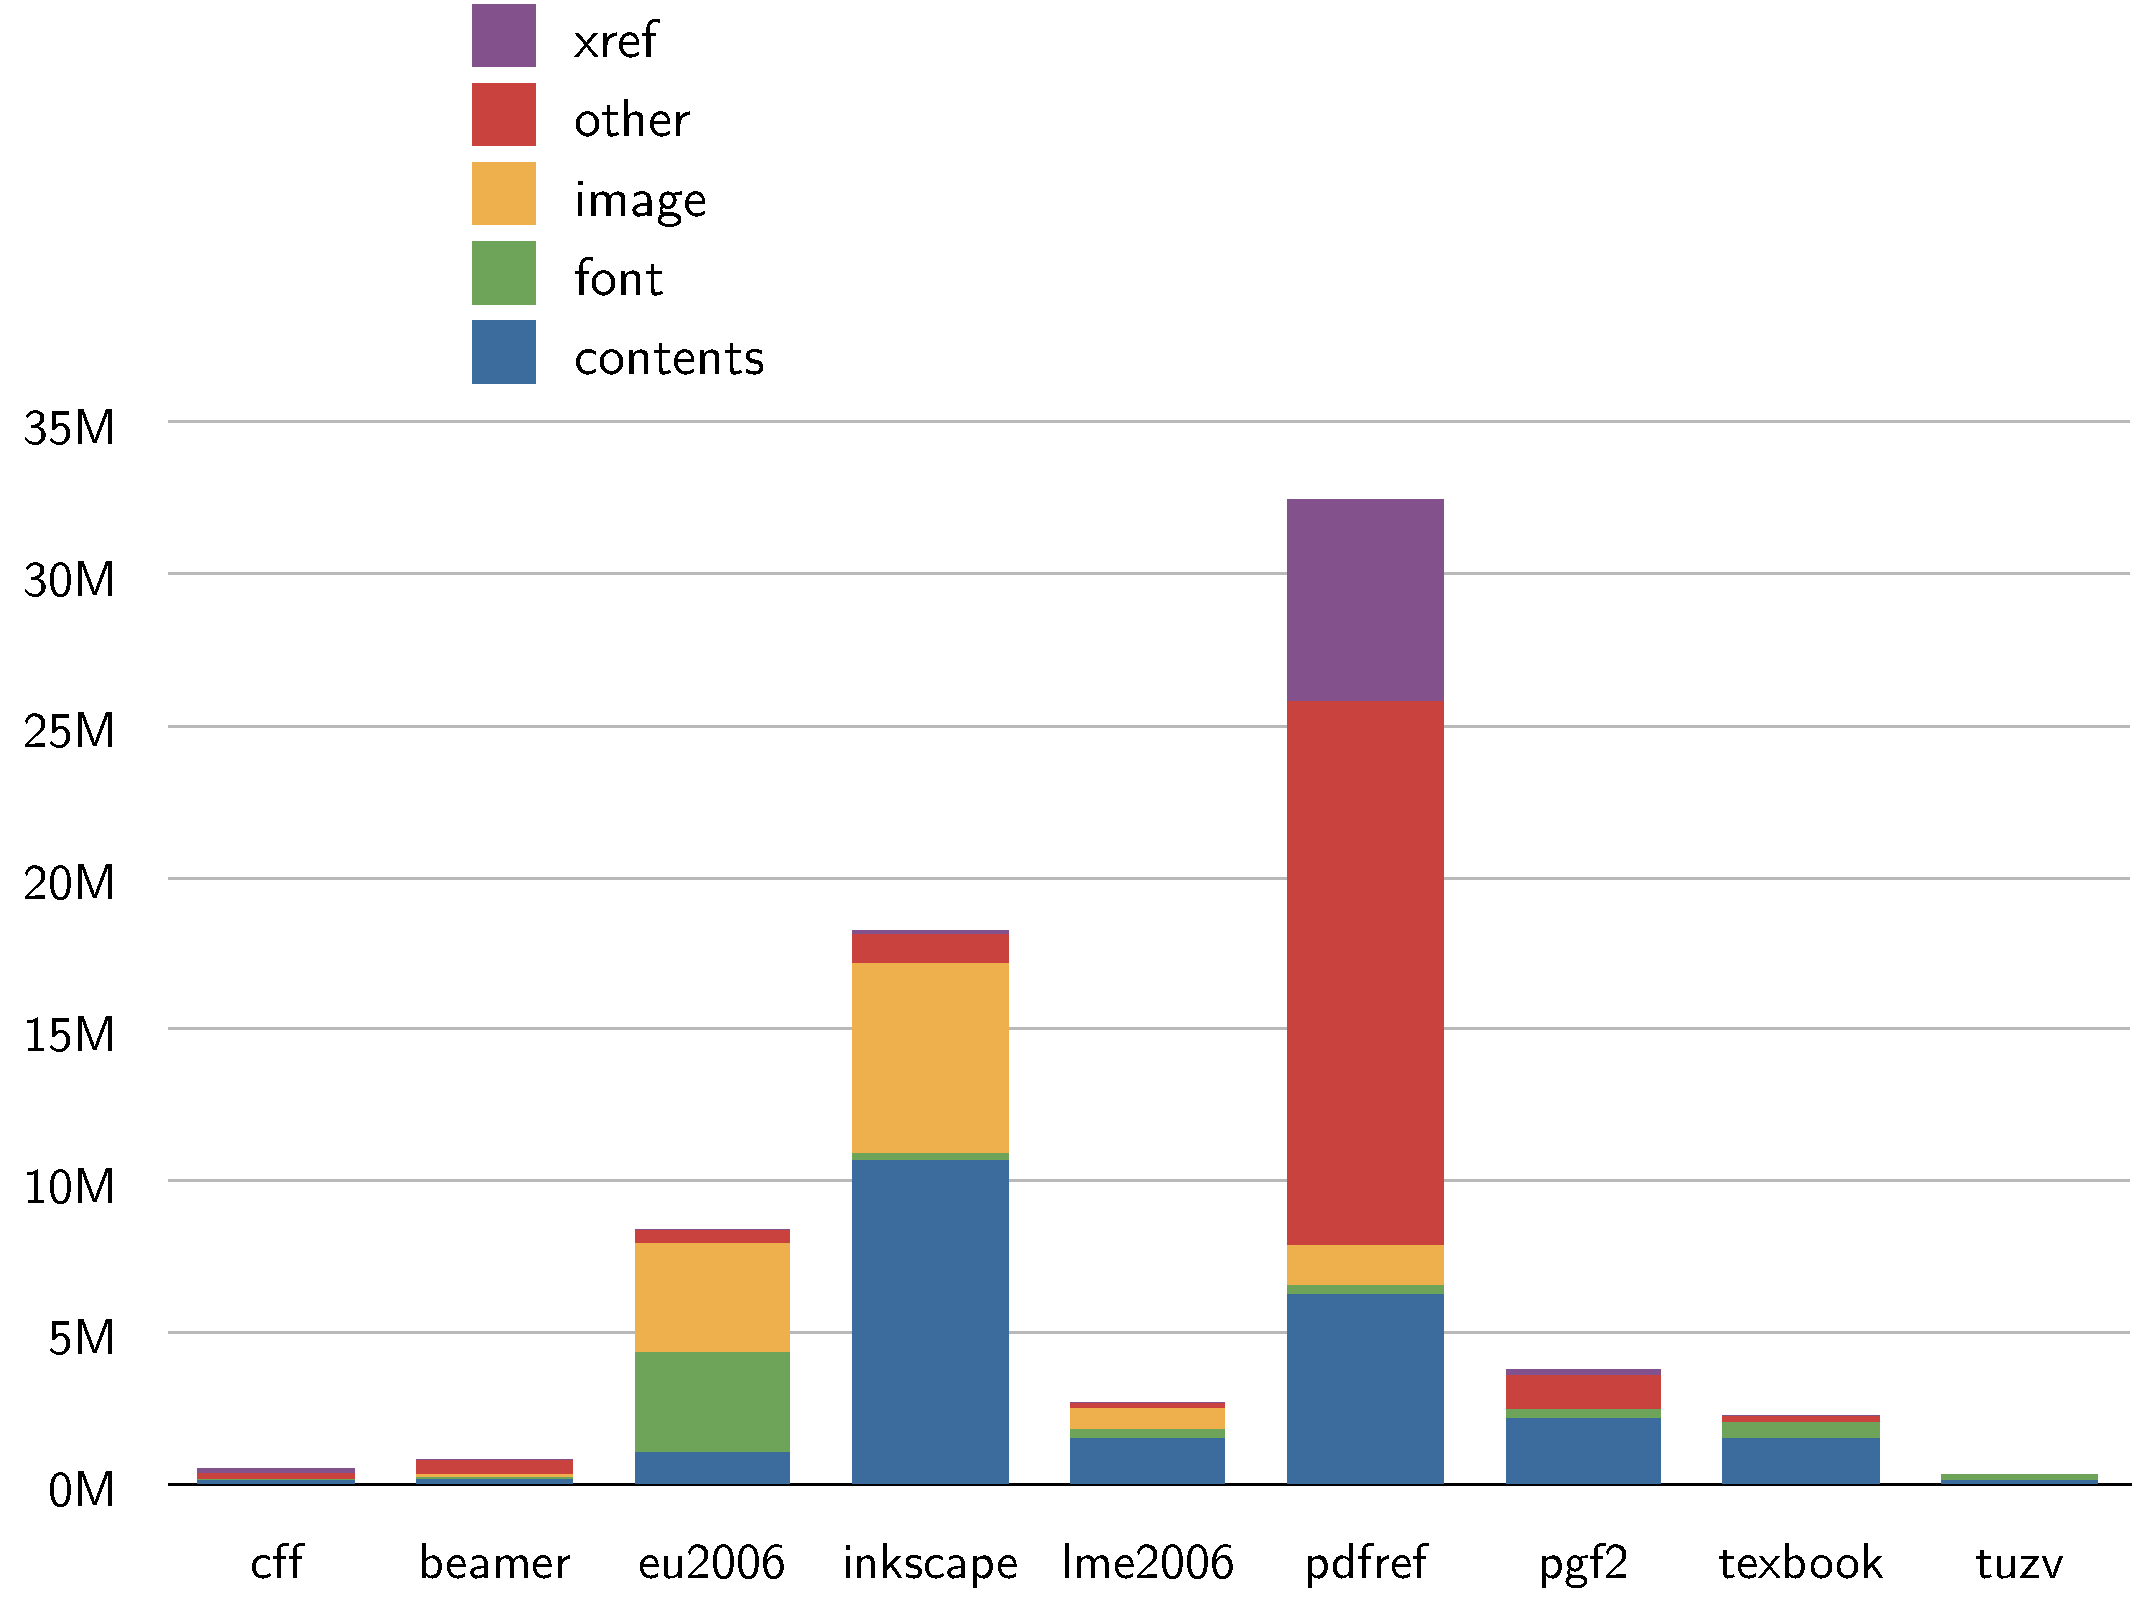
\includegraphics[height=\vsize]{pdfsizeopt_charts.pdf}
}}

\frame{
\frametitle{Input PDF feature distribution}
\nocenter{%
\noindent\hfil
\includegraphics[height=\vsize,page=2]{pdfsizeopt_charts.pdf}
}}

\subsection{Optimization effectiveness by feature}

\frame{
\frametitle{Image optimization effectiveness (byte sizes)}
\nocenter{%
\noindent\hfil
\includegraphics[height=\vsize,page=3]{pdfsizeopt_charts.pdf}
}}

\frame{
\frametitle{Vector graphics and text optimization effectiveness}
\nocenter{%
\noindent\hfil
\includegraphics[height=\vsize,page=4]{pdfsizeopt_charts.pdf}
}}

\frame{
\frametitle{Embedded font optimization effectiveness}
\nocenter{%
\noindent\hfil
\includegraphics[height=\vsize,page=5]{pdfsizeopt_charts.pdf}
}}

\frame{
\frametitle{Pixel image optimization effectiveness}
\nocenter{%
\noindent\hfil
\includegraphics[height=\vsize,page=6]{pdfsizeopt_charts.pdf}
}}

\frame{
\frametitle{Other data optimization effectiveness}
\nocenter{%
\noindent\hfil
\includegraphics[height=\vsize,page=7]{pdfsizeopt_charts.pdf}
}}

\frame{
\frametitle{Cross-reference optimization effectiveness}
\nocenter{%
\noindent\hfil
\includegraphics[height=\vsize,page=8]{pdfsizeopt_charts.pdf}
}}

\section{Discussion}
%\subsection{Overview of the Beamer Class}
\frame
{
  \frametitle{Features of the Beamer Class}

  \begin{itemize}
  \item<1-> Normal LaTeX class.
  \item<2-> Easy overlays.
  \item<3-> No external programs needed.      
  \end{itemize}
}
\end{document}
